\documentclass[a4paper,12pt,draft]{article}
\usepackage{a4wide}
\usepackage{ucs}
\usepackage[utf8x]{inputenc}
\usepackage{xcolor}
\usepackage[czech]{babel}
\usepackage[pdftex, final]{graphicx}
\usepackage[pdftex, final, colorlinks=true]{hyperref}
\usepackage{verbatim}
\usepackage{alltt}
\usepackage{mdwlist}
% \usepackage{stdpage}
\usepackage{subfig}
\parskip=0.8ex plus 0.4ex minus 0.1 ex


%%%%%%%%%%%%%%%%%%%%%%%%%%%%%%%
\usepackage[final]{listings}

\definecolor{lightGrey}{RGB}{250,250,250}
\definecolor{darkGrey}{RGB}{100,100,100}
\lstdefinelanguage{psmap}
{morekeywords={scale, mapinfo, maploc, where, end, font, fontsize, color, border, raster, width, paper,
vpoints, vareas, vlines, symbol, size, rgbcolumn, sizecolumn, cwidth, rotatecolumn, },
morekeywords=[2]{y, n, none},
morecomment=[l]{\#},
}
\lstdefinestyle{psmap}{
   language=psmap,
   basicstyle={\sffamily},
   keywordstyle=[1]{\bfseries},
   keywordstyle=[2]{\color{darkGrey}},
   commentstyle={\itshape},
   frame=lines,
   backgroundcolor=\color{lightGrey},
}
\lstdefinestyle{psmapInline}{
   language=psmap,
   basicstyle={\sffamily},
   keywordstyle=[1]{},
   keywordstyle=[2]{\bfseries\color{darkGrey}},
   commentstyle={\itshape},
   frame=lines,
   backgroundcolor=\color{lightGrey},
}
\lstnewenvironment{psmap}[1][]
{\lstset{style=psmap,
   #1}}
   {}

\newcommand{\modul}[1]{\emph{#1}}
\newcommand{\instr}[1]{\lstinline[style=psmapInline]|#1|}
\author{Anna Kratochvílová}


\begin{document}
\tableofcontents
\renewcommand{\refname}{Použité zdroje}

\section{Úvod}

\section{Programy pro tvorbu mapových výstupů}

Tvorba map dnes již dávno není pouze věcí specializovaných pracovišť. Rozvoj geografických informačních systémů natolik zjednodušil tvorbu mapových výstupů, že mapy, ať už jakékoli kvality, potkáváme na každém kroku. Různé formy map se staly moderním doplňkem v novinách, televizních zprávách, letácích a především na internetu, téměř každá informace má totiž vazbu na geografickou polohu.

Definic geografického informačního systému (dále jen GIS) existuje mnoho a další časem pravděpodobně ještě vzniknou, jak se bude tato oblast vyvíjet. Někteří odborníci v definicích vyzdvihují význam složky datové, jiní zas analytické, v souvislosti s tématem této práce je ale důležité především znázornění dat.

Existuje poměrně velké množství programů umožňujících tvorbu mapových výstupů. Většinou tato funkcionalita nestojí samostatně, ale je součástí většího GIS softwaru. Existující programy lze rozdělit podle mnoha kritérií, ale jedno z nejdůležitějších kritérií je určitě finanční dostupnost. Naštěstí v oblasti GIS existuje velký výběr open source programů, tedy programů, jejichž použití není zpoplatněno. Zdaleka zde neplatí myšlenka, že co je zdarma, je podezřelé a nefunguje. Komerční řešení sice často mají v některých oblastech širší funkcionalitu, ale ta může být samostatně zpoplatněna, případně může být implementována méně efektivním způsobem (například u algoritmů). Další výhodou open source projektů je dostupnost zdrojových kódů, což sice běžné uživatele nezajímá, ale pro odbornou veřejnost to znamená možnost si postrádanou funkčnost vlastními silami dopsat. Jedním z dalších argumentů mluvících pro open source software je rychlá odezva v případě jakýchkoli problémů. Při volbě vhodného softwaru je tedy třeba zvážit mnoho faktorů. Pro velké projekty je často vhodnější komerční program, který pokryje všechnu potřebnou funkcionalitu. Bohužel se dnes často stává, že velká komerční řešení se používají i tam, kde by plně postačil open source software, a to jen kvůli neznalosti.


\subsection{Porovnání možností programů pro tvorbu mapových výstupů}
V rámci práce na grafickém rozhraní pro modul \modul{ps.map} bylo vhodné se seznámit s funkcionalitou aspoň některých programů, které se používají pro mapové výstupy. Vzhledem k dostupnosti softwaru byl pro porovnání vybrán proprietární software \emph{ArcGIS 10.0} a
open source programy \emph{gvSIG 1.10}, \emph{Quantum GIS} verze \emph{1.6.0-Copiapo} a samozřejmě modul \modul{ps.map} systému \emph{GRASS GIS}.
Toto porovnání si neklade za cíl vytvořit kompletní seznam funcionality programů, což by bylo téma pro samostatnou práci, cílem je pouze zdůraznit některé zajímavé možnosti, které programy nabízí. Detailněji je pak popsán modul \modul{ps.map}, jehož možnosti bylo třeba zkoumat do nejmenších podrobností.

\subsubsection{ArcGIS}
Tento software od firmy \emph{ESRI} je jeden z nejpoužívanějších v České republice. ArcGIS sestává z několika základních aplikací,  pro tvorbu mapových výstupů slouží aplikace \emph{ArcMap}.

Při práci v programu je třeba rozlišit dva módy -- \emph{Data View} a \emph{Layout View}. Data View slouží pro běžnou práci s daty, zatímco Layout View je použit pro vytvoření mapového výstupu, zobrazuje výřez mapy na stránce. Tyto dva módy jsou propojené a změny se projevují v obou. V Layout View lze zobrazit vodící linky a mřížku pro přesnější pozicování  a  přidávat mapové elementy: legenda, měřítko grafické a číselné, směrovou růžici, titulek, text, dynamický text, rámeček, obrázek, jiný objekt (tabulku, graf).  Možnosti nastavení vlastností pro jednotlivé prvky je velice široké, což umožňuje uzpůsobit mapový výstup svým představám. Při velkém množství dat je pro urychlení práce vhodné nevykreslovat objekty, ale zobrazovat je pouze jako šedé obdélníky s popisem (\emph{Draft mode}), toto řešení je dostupné i v jiných programech. ArcMap dovoluje poměrně pokročilou práci s vektorovou grafikou, lze kreslit základní tvary, seskupovat je, zarovnávat, rotovat či měnit jejich hladinu.

Většinu výše jmenovaných funkcionalit mají i jiné takto specializované programy. Co již tak běžné není, je použití více datových rámců (\emph{Data Frame}), například QGIS tuto funkcionalitu neposkytuje. Důsledkem je možnost umístit na stránku více mapových rámců (výřezů) zobrazujících \emph{různá} data. Tato vlastnost se vyžívá, chceme-li například zobrazit centrum města ve větším měřítku a méně generalizované než je zbytek mapy. 

Další zajímavou vlastností je tvorba šablon pro mapové výstupy a s tím souvisí i tzv. \emph{Řízené mapové listy} neboli \emph{Data Driven Pages}. Tímto nástrojem lze najednou vygenerovat sadu mapových výstupů. Například pro data obsahující okresy ČR lze velice jednoduše vytvořit sadu stejně vypadajících mapových výstupů zobrazujících jednotlivé okresy.


\subsubsection{gvSIG}
GIS gvSIG je open source software šířený pod licencí GNU/GPL. Je lokalizovaný do mnoha jazyků včetně češtiny a dostupný na všech běžných platformách (Linux, MS Windows, Mac OS X). Existuje i produkt gvSIG Mobile určený pro použití v mobilních zařízeních. gvSIG je napsán v programovacím jazyce Java, díky čemuž má mnoho aktivních vývojářů.

Projekt programu gvSIGu sestává tří hlavních částí -- \emph{View}, \emph{Table} a \emph{Map}, v poslední jmenované pak probíhá tvorba mapových výstupů. View je obdobou datového rámce v ArcGISu. Na stránku lze tedy umístit více mapových rámců, u každého se pak zvolí, který View bude zobrazovat. Podporované mapové elementy jsou obdobné jako u ArcGISu, navíc umí gvSIG přímo vložit lokalizační mapku, to je sice u ArcGISu také možné, ale tato funkce není tak jednoduše přístupná. Drobné rozdíly najdete v možnostech nastavení vzhledu jednotlivých elementů, ale opravdu není podstatné, jestli máte na výběr mezi 50 nebo 100 různých směrových růžic. Co mne trochu zklamalo, byla legenda, jejíž vlastnosti se poměrně špatně nastavovaly. Pro více sloupců je potřeba ji nejprve rozložit na jednotlivé grafické elementy a pak s ní pracovat jako s vektorovou grafikou. Co se týče exportních formátů, gvSIG podporuje pouze PS a PDF, zatímco ArcGIS má daleko širší výběr. To ale dnes není tak důležité vzhledem k existujícím grafickým editorům, které jsou schopné načíst a konvertovat velké množství formátů.

\subsubsection{QGIS}
Quantum GIS je rychle rostoucí GIS projekt psaný v C++, je opět šířený pod licencí GNU/GPL. Pro tvorbu mapových výstupů slouží \emph{Map Composer}, jehož funkcionalita plně nedosahuje úrovně programů ArcGIS ani gvSIG, nicméně pro ne příliš sofistikované mapové výstupy je to výborný prostředek.

Map Composer umožnuje sice vložit více mapových rámců, ale zobrazují pouze stejná data. Lze přidat standardní mapové elementy jako měřítko, legenda, text, atributovou tabulku, obrázek, jednoduché tvary. Směrová růžice se přidává v rámci obrázků. Zajímavou vlastností je přidání atributové tabulky pro zvolenou mapovou vrstvu, z tabulky se dají vybrat pouze některé atributy a také lze vhodně záznamy seřadit. Tuto funkcionalitu z porovnávaných programů poskytuje pouze ArcGIS, ale nastavení vlastností tabulky zde už není tak jednoduché. Legenda pro vektorové vrstvy se chová standardně, ale pro rastr v podstatě nefunguje. Pro pozicování objektů je k dispozici mřížka s nastavitelnými parametry a volitelným přichytáváním. Dobře funguje i zobrazení souřadnicové sítě s popisky.



\subsubsection{GRASS GIS -- ps.map}
\label{sec:porovnani:psmap}
GRASS GIS (viz část \ref{sec:grass} na straně \pageref{sec:grass}) jakožto významný představitel open source geografických informačních systémů má v tvorbě mapových výstupů značné rezervy. Prakticky jediným vhodným nástrojem, kterým GRASS GIS v současnosti disponuje, je modul \modul{ps.map}\footnote{V současné době je vyvíjen modul \modul{ps.output}, který rozšiřuje možnosti \modul{ps.map} a možná jej v budoucnu nahradí, nicméně zatím je k dispozici jen v grass-addons.}.

Pro uživatele je základním rozdílem mezi \modul{ps.map} a ostatními programy pro tvorbu mapových výstupů  absence grafického uživatelského rozhraní. To je pro většinu uživatelů velký problém, částečně proto není tento modul příliš využívaný. Mapový výstup je ovládán konfiguračním souborem, což je obyčejný textový soubor s instrukcemi, co se má kam vykreslit. Po technické stránce je tento modul podrobněji  popsán v oddíle \nameref{sec:psmap}.

Dalším výrazným rozdílem je oddělenost tvorby mapového výstupu od zbytku programu. To se projevuje tím, že je nutné explicitně uvést všechny mapové vrstvy, které se mají zobrazit, a také nastavit jejich vzhled, nehledě na mapové vrstvy aktuálně zobrazované  v grafickém uživatelském prostředí GRASSu.

Modul \modul{ps.map} nepodporuje češtinu, což je dáno použitým kódováním. \modul{Ps.map} očekává konfigurační soubor v kódování Latin-1 (přesněji ISO-8859-1), které není pro češtinu použitelné kvůli některým chybějícím znakům s diakritikou. Navíc některé texty (například jednotky u grafického měřítka) jsou v angličtině.

Mapový výstup \modul{ps.map} obsahuje většinu standardních prvků jako legenda, měřítko apod. Možnosti nastavení jejich vzhledu nejsou tak široké jako u jiných programů, což v některých případech nevadí.

\paragraph*{Mapový rámec}
Nevýhodou \modul{ps.map} je chybějící podpora pro více mapových rámců. V jednom mapovém výstupu lze tak zobrazit pouze jednu oblast\footnote{Toto omezení se dá obejít vložením EPS souboru s mapou, ale to není dostatečně komfortní řešení.}. Dalším omezením je vykreslení maximálně jedné rastrové mapy (případně složené 3 vrstvy jako RGB). Vektorových map lze nicméně přidat libovolný počet. Lze u nich nastavit vzhled (symboly, styl čáry, barevnost, výplň, ...) a také například omezit zobrazené prvky atributovým dotazem.

V mapovém rámci lze dále zobrazit zeměpisnou síť (grid), popisky (labels) nebo zvýraznit uložený region s menším rozsahem.

\paragraph*{Legenda}
Vzhled legendy \modul{ps.map} se v zásadě příliš neliší od ostatních programů. V podstatě jediným podstatnějším rozdílem je fakt, že \modul{ps.map} striktně rozlišuje rastrovou a vektorou legendu. Jde o dva oddělené objekty, což není obvyklé a asi ani žádoucí řešení. Vzhled rastrové legendy závisí na typu dat, je buď spojitá, nebo rozdělená podle kategorií, to je běžné i v ostatních programech.

\paragraph*{Měřítko}
Je třeba odlišit grafické a číselné měřítko, opět jde o dva odlišné objekty.
U grafického měřítka sice modul nenabízí takové množství různých stylů (pouze dva) jako např. ArcGIS, nicméně stojí za zmínku způsob, jakým se určuje velikost měřítka. Jeho délka je totiž dána zadanou délkou v mapových jednotkách. Podobný způsob sice ArcGIS, QGIS i gvSIG umožňují také, ale zvláště v případě ArcGISu je pro uživatele těžké se v nastavení vyznat a vybrat to správné. U \modul{ps.map} proto můžeme považovat jednoduchost nastavení za výhodu, pro většinu mapových výstupů navíc jednoduchý vzhled grafického měřítka postačuje.

Klasické číselné měřítko modul nenabízí. Je totiž součástí objektu \emph{mapinfo}, který obsahuje informace o aktuálním zobrazovaném regionu, zobrazované zeměpisné síti a měřítku, viz obr. č. \ref{fig:mapinfo}. Mapinfo nemá v ostatních programech obdobu, snad kromě ArcGISu, kde lze podobně zobrazit informace o souřadnicovém systému pomocí automaticky generovaného textu (\emph{Dynamic text}). 
\begin{figure}[h!]
    \centering
    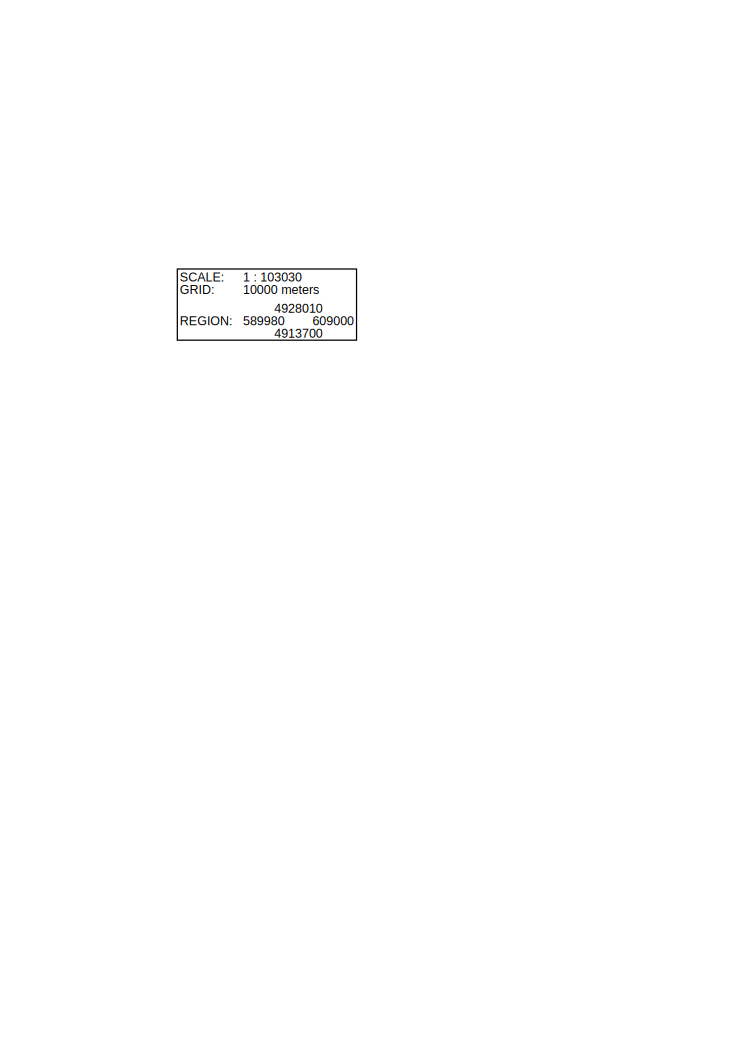
\includegraphics[width=0.2\textheight]{./mapinfo.pdf}
    \caption{Mapinfo}
    \label{fig:mapinfo}
\end{figure}

\paragraph*{Směrová růžice}
Symbol severu v modulu \modul{ps.map} vůbec není k dispozici, což je velkou nevýhodou, jelikož určení severu je v mapových výstupech obvyklé. Tento problém lze řešit buď přidáním obrázku ve formátu EPS, případně lze šipku vytvořit složením z jiných grafických objektů (postup lze najít na webové stránce \cite{wiki_psmap_north}).

\paragraph*{Další možnosti}
Modul dále umožňuje kreslit základní tvary jako obdélník, linii a bod. K mapovému výstupu lze připojit hlavičku, kde jsou uvedeny základní informace o mapě. Text hlavičky je uložen v externím souboru, používá speciální formátovací značky pro vložení aktuálního data, názvu rastru, lokaci apod. Jinak samozřejmě mapový výstup může obsahovat jakékoli množství textu, ten lze různě barevně zvýrazňovat. Texty lze modulem \modul{ps.map} umisťovat na konkrétní pozici zadáním mapových souřadnic, což ostatní programy nepodporují. 




\subsection{Porovnání programů pro tvorbu mapových výstupů z hlediska uživatelského rozhraní }
\subsubsection{Obecné zásady grafického uživatelského rozhraní}
\subsubsection{ArcGIS}

\subsubsection{QGIS}

\subsubsection{gvSIG}



\subsubsection{GRASS -- wx.psmap}

\subsection{Výsledek porovnání}
Je důležité, aby software pro mapové výstupy splňoval poměrně konzervativní kartografické zásady, a na to nejsou potřeba desítky různých nastavení. Příliš široké možnosti vedou ke komplikovanějšímu grafickému rozhraní a tedy k horší ovladatelnosti a navíc podněcují nezkušené uživatele, aby vyzkoušeli a použili všechna dostupná nastavení, což posléze vede k překombinovanému a nevkusnému výsledku.


\section{Systém GRASS GIS}
\label{sec:grass}
GRASS GIS (Geographical Resources Analysis Support System) je jedním z nejrozsáhlejších \emph{Free Software}\footnote{\url{http://www.gnu.org/philosophy/free-sw.html}} geografických informačních systémů, publikovaných pod licencí \emph{GNU General Public Licence}\footnote{\url{http://www.gnu.org/licenses/gpl.html}}. Obsahuje více než 350 modulů pro správu prostorových dat, zpracování obrazových dat z leteckých a družicových snímků, analýzu a vizualizaci dat rastrových a vektorových. GRASS GIS je vyvíjen jazyce C a je multiplatformní.

GRASS GIS je projektem s dlouhou historií. Byl původně vyvíjen od roku 1982 laboratořemi v USA (\emph{USA-CERL}) pro vojenské účely. Koncem 80. let poskytl CERL zdrojové kódy veřejnosti a GRASS se během několika let rozšířil po celém světě. Vývoj převzaly \emph{Baylor University} v Texasu, \emph{Universtät Hannover} a další pod souhrnným názvem \emph{GRASS Development Team}. V roce 1998 byla uvolněna verze GRASS 4.2.1 a v současnosti je poslední uvolněnou verzí GRASS 6.4. Vývoj nyní probíhá na nejnovější verzi GRASS 7, která sice ještě není připravená k uvolnění, ale je funkční. 

Pro více informací o vývoji, funkčnosti a použití GRASS GIS nahlédněte do knihy \cite{grass_gis} nebo na stránky \cite{grass_page}.

\subsection{Základní pojmy}
\label{sec:grass:pojmy}
Jelikož jsou v dalším textu použity některé pojmy specifické pro GRASS, je třeba je alespoň trochu přiblížit čtenářům bez předchozích znalostí systému GRASS. Tyto pojmy souvisí především se strukturou dat, kterou GRASS používá.

\begin{description}
\item[Database] neboli databanka představuje adresář s obvyklým názvem \emph{grassdata}, který obsahuje veškerá data, se kterými GRASS pracuje.
\item [Location] neboli lokace je adresář nacházející se v databance. Určen je souřadnicovým systémem a územním rozsahem. Jedna lokace většinou odpovídá jednomu projektu.
\item [Mapset] je soubor map (rastrové, vektorové, \ldots) v rámci jedné lokace. Jedna lokace obsahuje minimálně jeden mapset s názvem PERMANENT, který  slouží jako zdroj dat pro další mapsety, které jsou pracovní. Tyto mapsety zpravidla odpovídají jednotlivým uživatelům, případně různým analýzám.
\item [Region] určuje územní rozsah ve tvaru obdélníka a také rozlišení, které se uplatní pouze u rastrových map. Jde o klíčový pojem, protože při práci v GRASSu je třeba nastavení regionu často řešit.  Rozlišujeme výchozí region (pro celou lokaci) a aktuální (výpočetní) region. Téměř veškeré manipulace s daty se pak týkají aktuálně nastaveného regionu. K nastavení regionu slouží modul \emph{g.region}, umožní nastavit region podle konkrétní mapy, přímým zadáním hraničních souřadnic, nebo z již uloženého regionu (\emph{named region}). 
 \end{description}

\subsection{Instalace systému GRASS GIS}
Instalace systému GRASS GIS je závisí na jeho verzi a operačním systému. Stručně popíši způsob instalace na operační systém Linux (distribuci Ubuntu), podrobnosti k instalaci i na ostatních systémech (MS Windows a Mac OS X) je popsána na GRASS-Wiki \cite{instalace}.

Nejjednodušší je nainstalovat stabilní verzi GRASS 6.4, která je dostupná v balíčku. Lze ji proto nainstalovat pomocí správce balíčků \emph{Synaptic}. Nebo do příkazové řádky napsat:
\begin{alltt}
{\footnotesize sudo apt-get install grass grass-doc}
\end{alltt}

Nové grafické rozhraní pro modul \modul{ps.map} je funkční pro verze 6.5 a vyšší. Ty nejsou dostupné v balíčku, ale lze je nainstalovat jinak, i když ne tak jednoduše. První možnost je stáhnout binární soubory  a spustit instalační skript. Tyto soubory jsou týdně aktualizovány. Pokud chcete i zdrojový kód, lze si soubory stáhnout z repozitáře SVN, a to buď formou tzv. \emph{SVN snapshot} bez založení lokálního repozitáře nebo se založením lokálního repozitáře pomocí následujících příkazů:
\begin{alltt}
{\footnotesize
svn checkout https://svn.osgeo.org/grass/grass/branches/develbranch_6 grass6_devel}
\end{alltt}
pro verzi 6.5 a pro verzi 7:
\begin{alltt}
{\footnotesize
svn checkout https://svn.osgeo.org/grass/grass/trunk grass_trunk}
\end{alltt}
Tato možnost má tu výhodu, že po instalaci lze jednoduše provádět aktualizaci pomocí \verb|svn up|. Postup instalace je následující: ve vybraném adresáři (například \verb|/usr/local/src|) s právem zápisu spustťe výše uvedený příkaz a po stažení repozitáře pokračujte spuštěním
\begin{alltt}
{\footnotesize ./configure}
\end{alltt}
Velmi pravděpodobně skript skončí předčasně kvůli chybějící knihovně. Je třeba se podívat, zda je na počítači instalován veškerý vyžadovaný software\footnote{\url{http://grass.osgeo.org/grass64/source/REQUIREMENTS.html}} a pokud ne, pak jej doinstalovat (nejlépe pomocí balíčků). Téměř úplný seznam nutných balíčků:
\begin{alltt}
{\footnotesize
flex, bison, libreadline5-dev | libreadline-dev, libncurses5-dev, lesstif2-dev, 
debhelper (>= 5), dpatch, libtiff4-dev, tcl-dev (>= 8.4) | tcl8.4-dev, 
tk-dev (>= 8.4) | tk8.4-dev, libfftw3-dev|fftw3-dev, libxmu-dev, 
libglu1-mesa-dev | libglu1-xorg-dev, libfreetype6-dev, autoconf2.13, 
autotools-dev, libgdal1-dev (>=1.4.0) | libgdal1-1.3.2-dev, proj (>= 4.4.7),
libjpeg62-dev, libpng12-dev, libpq-dev, unixodbc-dev, doxygen, fakeroot, 
libmysqlclient15-dev, graphviz, libsqlite3-de
}
\end{alltt}
Může nastat problém ve špatně nastavené cestě ke knihovnám, pro jejich nalezení poslouží příkaz \verb|locate|. Cesty lze nastavit v parametrech skriptu configure. Pro nápovědu použijte \verb|./configure -- help|. Správnou cestu lze pak nastavit například takto:
\begin{alltt}
{\footnotesize./configure --with-freetype-includes=/usr/include/freetype2   }
\end{alltt}

Po korektním skončení \verb|configure| následuje kompilace pomocí \verb|make|, což chvíli potrvá. Pokud skončí bez chyb, instalace je dokončena pomocí \verb|make install|. 


\subsection{Grafické rozhraní systému GRASS GIS}
Původně bylo zamýšleno, že systém GRASS GIS bude ovládán z příkazové řádky, ostatně v dobách jeho vzniku nemohla být o něčem jiném ani řeč. Nicméně postupem času vzrůstal ze strany uživatelů tlak na vytvoření grafického rozhraní. První GUI nazývané \emph{TCLTKGRASS} bylo napsáno v roce 1999 v programovacím jazyce \emph{Tcl} s využitím knihovny \emph{Tk}. Nástupcem byly v dalších verzích GRASS 6 \emph{Display Manager} a poté \emph{GIS Manager}, stále napsané pomocí Tcl/Tk. Vzhledem k omezením Tcl/Tk bylo rozhodnuto přepsat grafické rozhraní pomocí modernější knihovny. Po zvážení různých aspektů (přenositelnost, dostatečná funkcionalita, oblíbenost u vývojářů) byl vybrán \emph{wxPython}, který obaluje knihovnu \emph{wxWidgets}, implementovanou v C++. Nové GUI je tedy napsáno v programovacím jazyce Python. 

Nové grafické rozhraní \emph{wxGUI} bylo vyvíjeno od roku 2006 a je dostupné od verze 6.4. Skládá se ze dvou hlavních komponent -- \emph{Layer Manager} a \emph{Map Display Window}, viz obr. č. \ref{fig:wxgui}. Layer Manager spravuje mapové vstvy, umožňuje spouštět GRASS moduly a zobrazuje výstup programů. Map Display Window především zobrazuje mapové vrstvy a ovládá pohled (přiblížení, posunutí). Většina modulů se ovládá prostřednictvím dialogů generovaných z XML popisu jejich rozhraní, některé mají své samostatně vytvořené dialogy.
\begin{figure}[h!]
\centering
\subfloat[][Layer Manager]{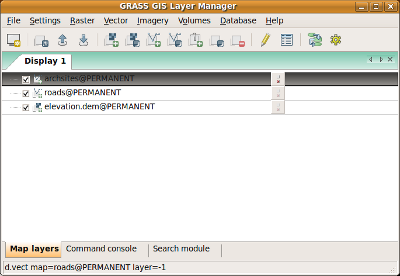
\includegraphics[width=0.45\textwidth]{./wxgui_layer_manager.png}}   \quad              
\subfloat[][Map Display Window]{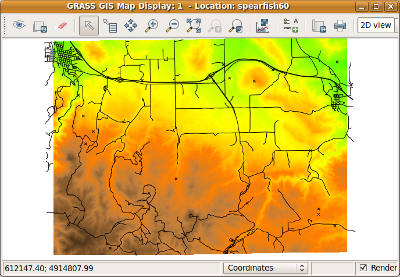
\includegraphics[width=0.45\textwidth]{./wxgui_map_display.png}}  
\caption{Dvě hlavní komponenty wxGUI v GRASS 7\label{fig:wxgui}}

\end{figure}

\subsection{Modul ps.map}
\label{sec:psmap}
Modul \modul{ps.map} je v současnosti nejvhodnější prostředek pro tvorbu mapových výstupů v GRASSu. Další alternativou je zobrazit si potřebné mapové vrstvy v mapovém okně (Map Display Window)  a upravit jejich vzhled, případně zobrazit i legendu či měřítko. Zde jsou možnosti poměrně omezené, navíc lze výstup uložit pouze jako rastrový obrázek a celkově tento způsob není příliš vhodný pro tvorbu mapového výstupu.

Modul \modul{ps.map} lze jako většinu modulů používat z příkazové řádky GRASSu nebo pro\-střed\-nic\-tvím wxGUI. Grafické rozhraní je vytvořeno stejným způsobem jako u většiny ostatních modulů, dovoluje tedy zadat parametry příkazu v dialogu. V tomto případě ale spouštění přes grafické rozhraní neskýtá mimořádnou výhodu, jelikož v zásadě většinou stačí zadat jméno již připraveného konfiguračního souboru a souboru výstupního, což je pro mnohé uživatele pohodlnější prostřednictvím příkazové řádky. V příkazové řádce vypadá spuštění \modul{ps.map} takto:
\begin{verbatim}
 ps.map input=/konfiguracni/soubor.txt output=/vystupni/soubor.ps   
\end{verbatim}

Jak již bylo zmíněno v části \ref{sec:porovnani:psmap}, modul vytváří mapový výstup na základě konfiguračního souboru, což je obyčejný textový soubor s instrukcemi. Vytvořit tento soubor je většinou poměrně pracné, umisťování mapových prvků na vhodnou pozici se často neobejde bez vedlejších výpočtů, což ke konformitě používání příliš nepřispívá. Z toho je zřejmé, že v současnosti \modul{ps.map} využívá pouze poměrně úzká komunita uživatelů GRASSu. Nové grafické rozhraní \emph{wx.pasmap} přímo vytváří konfigurační soubor, na základě něhož poté \modul{ps.map} vygeneruje mapový výstup. Není pak třeba se konfiguračním souborem zabývat, což může zpříjemnit používání tohoto modulu, a tím i rozšířit řady jeho uživatelů. 

\subsubsection{Konfigurační soubor}
Konfigurační soubor má poměrně jednoduchou strukturu. Skládá se z instrukcí, které musí být na samostatných řádcích. Instrukce mohou obsahovat další dílčí instrukce umístěné opět na samostatných řádcích. Tyto víceřádkové instrukce musí být ukončeny  instrukcí \instr{end}, která musí být uvedena i na konci celého konfiguračního souboru. Dílčí instrukce je možné ve většině případů vynechat a pro nastavení dané vlastnosti se použije implicitní hodnota. Komentáře lze zapisovat pomocí znaku \#, prázdné řádky jsou ignorovány. Pořadí instrukcí většinou nehraje roli s výjimkou instrukcí \instr{vpoints}, \instr{vlines} a \instr{vareas}, které vykreslují vektorové vrstvy. První uvedená vektorová vrstva bude vykreslena nejvýše. Více napoví ukázka jednoduchého konfiguračního souboru:
\begin{psmap}
paper a3
end
raster soils            # priklad jednoradkove instrukce
border y                # priklad viceradkove instrukce ...
   color 255:0:0
   width 3
end                     # ... ukoncene instrukci end
vpoints archsites
   symbol basic/diamond
   size 10
end
end                     # konec instrukci
\end{psmap}
Význam jednotlivých instrukcí je popsán v manuálové stránce k modulu, která je dostupná buď z dosavadního GUI nebo na internetových stránkách \cite{manual}.

\subsubsection{Volba rozsahu zobrazovaného území}
\label{sec:psmap:rozsah}
V konfiguračním souboru lze nastavit velikost mapového rámce, čímž je myšlen obdélník s vykreslenou rastrovou či vektorovou mapou.  K nastavení slouží jednořádková instrukce \instr{maploc}, která umístí levý horní roh rámce na dané místo a volitelně nastaví i šířku a výšku mapového rámce. Rozměry lze nepřímo ovlivnit také instrukcí \instr{scale}, která na základě měřítka upraví rozměry rámce.

Nicméně při jakýchkoli rozměrech a umístění mapového rámce, se vykresluje stále stejný územní rozsah. Ten je dán tzv. \emph{výpočetním regionem}. Proto je třeba před vlastním generováním mapového výstupu nastavit výpočetní region tak, aby odpovídal území, které chceme zobrazit. K tomu slouží modul \modul{g.region}. V konfiguračním souboru tedy nelze rozsah území ovlivnit.
Modul \modul{ps.map} tedy nejprve zjistí požadované rozměry a měřítko z konfiguračního souboru (jsou-li uvedeny) a následně se je pokusí aplikovat na rozměry současného výpočetního regionu. Když by se mapový rámec při požadovaném měřítku nevešel na daný formát papíru, modul měřítko upraví. Podobně upraví rozměry mapového rámce, aby se vešel do zadaných rozměrů.

Nové grafické rozhraní wx.psmap řeší volbu zobrazovaného území ve vlastní režii, není tedy třeba volat modul \modul{g.region} a zároveň se nemění současný výpočetní region pro ostatí moduly. %Více v oddíle 

\subsubsection{Nekonzistence a chyby v modulu ps.map}
\label{sec:psmap:chyby}
Při tvorbě grafického rozhraní bylo nutné prozkoumat chování modulu \modul{ps.map} o něco detailněji, než je nutné pro jeho běžné užívání. Vycházela jsem především z manuálové stránky \cite{manual} a vlastního experimentování s modulem. 

\paragraph*{Souřadnicové systémy a jednotky}
\label{sec:psmap:sour_systemy}
Jedním z nejnepříjemnějších problémů, se kterými bylo třeba se při tvorbě GUI vypořádat, byla nekonzistence v jednotkách a souřadnicových sytémech. Modul \modul{ps.map} totiž pro umístění jednotlivých prvků (jako legenda, text, měřítko) používá dva různé systémy, viz obr. č. \ref{fig:sour_systemy}.

\begin{figure}[h!]
    \centering
    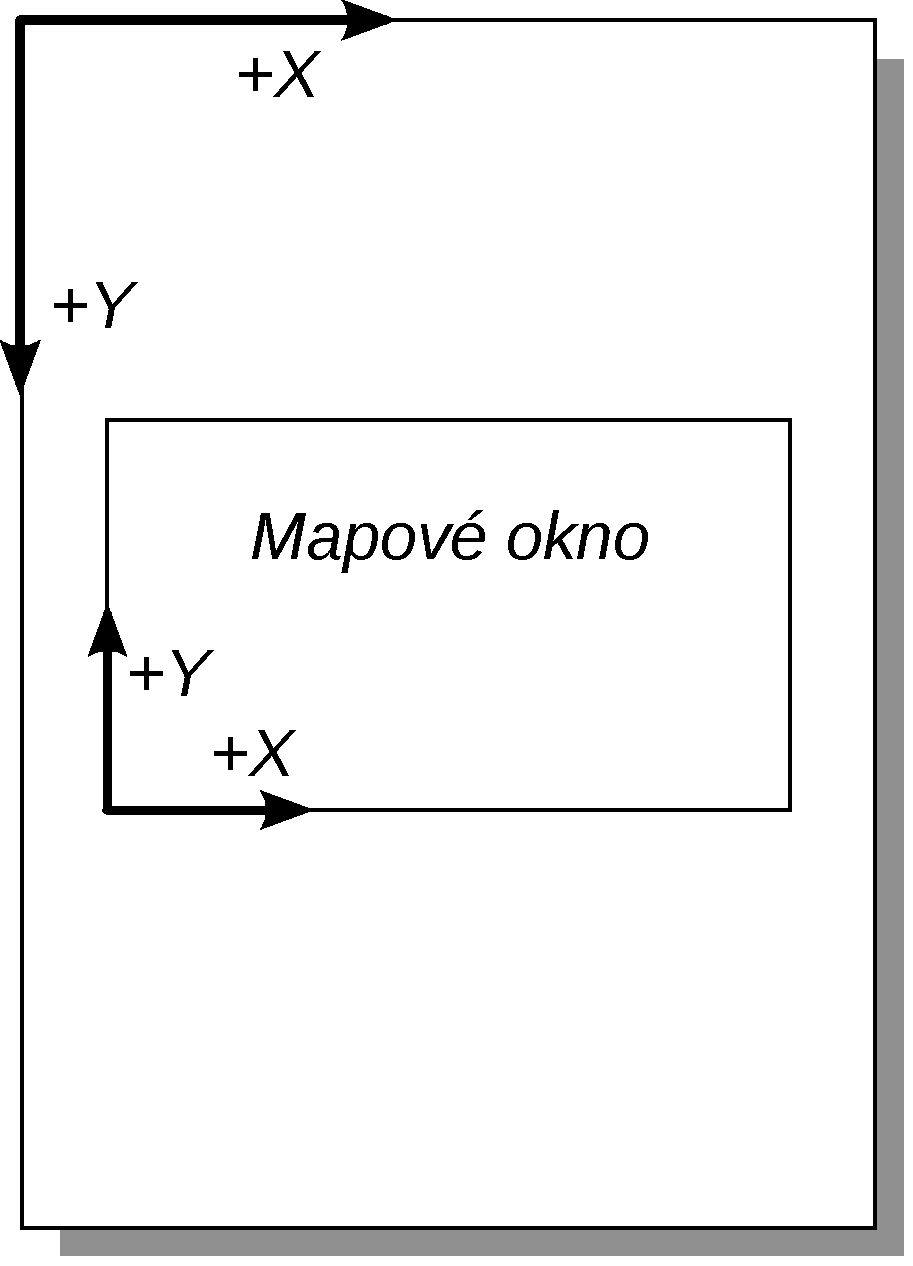
\includegraphics[width=0.2\textheight]{sour_systemy.pdf}
    \caption{Souřadnicové systémy používané modulem \modul{ps.map}\label{fig:sour_systemy}}
\end{figure}


První z nich -- souřadnicový systém papíru -- má počátek v levém horním rohu, kladná osa \emph{x} směřuje doprava a osa \emph{y} směrem dolů (tedy odpovídá systému obvyklému v počítačové grafice). 
Je-li poloha určena v tomto sytému, očekávanou jednotkou je inch\footnote{ česky palec, odpovídá $2{},54$ cm}.

Druhý systém -- systém mapového rámce -- má počátek souřadnic v levém dolním rohu mapového rámce s pravotočivou orientací os obvyklou v matematice. Souřadnice lze v tomto systému zadávat dvěma způsoby. Buď v procentech výpočetního regionu nebo přímo v souřadnicích mapy. Například, při souřadnicích [100\%, 0\%] je objekt umístěn v pravém dolním rohu mapového rámce, ať už je mapový rámec na papíře umístěn kdekoli. Alternativně bychom toho samého umístění dosáhli zadáním mapových souřadnic bodu položeného co nejvíce na východ a jih v rozsahu výpočetního regionu. Oběma způsoby lze dosáhnout i umístění objektu mimo mapový rámec, a to zadáním záporné hodnoty nebo hodnoty větší než 100 u procent, případně mapových souřadnic mimo výpočetní region.

Různé způsoby určení polohy mají své opodstatnění. V některých případech je výhodné umístit popisek k určitému místu, jehož mapové souřadnice známe, a jeho poloha vzhledem k papíru není podstatná. Pozicování pomocí procent je vhodné například pro nadpis mapy, který chceme umístit přesně doprostřed nad mapový rámec. 

Problém nastává v případě, když chce uživatel určit polohu objektu relativně k papíru a tento objekt podporuje umístění pouze relativně k mapovému rámci, případně naopak. Bylo by proto vhodné, aby všechny objekty podporovaly umístění všemi těmito způsoby. Uživatel by si pak mohl vybrat, který z nich je pro danou situaci nejvhodnější.

\paragraph*{Referenční bod objektu}
\label{sec:psmap:referencepoint}
Modul \modul{ps.map} u většiny objektů nepodporuje volbu referenčního bodu, tedy bodu objektu, ke kterému se vztahuje zadaná poloha. Výjimkou je text, u nějž si lze vybrat jeden z devíti referenčních bodů. Je zřejmé, že u textu má tato volba smysl, u ostatních objektů je otázka, zda by tato vlastnost byla využívaná. 
U ostatních objektů je referenční bod dán a nelze měnit. Uživatele však může překvapit, že není u všech objektů stejný. Ve většině případů se poloha vztahuje k levému hornímu rohu objektu, nicméně grafické měřítko (instrukce \instr{scalebar}) má referenční bod ve středu. Bylo by vhodné tento přístup sjednotit, na druhou stranu nejde o nijak zásadní problém. 

\paragraph*{Volba barev}
\label{sec:psmap:color}
V mnoha instrukcích se vyskytuje nastavení barvy. Bohužel velká část instrukcí omezuje výběr barev tím, že vyžaduje zadat barvu ve formě jejího jména, tedy např. \emph{aqua}, \emph{black}, \emph{blue}, \ldots Některé jiné instrukce však umožňují zadat barvu i ve tvaru R:G:B. Bylo by proto logické, kdyby RGB podporovaly všechny instrukce\footnote{Tyto problémy jsou již v současnosti vyřešené, alespoň pro instrukce, které wx.psmap podporuje}. 

\paragraph*{Jednořádkové a víceřádkové instrukce}
\label{sec:psmap:singleline}
Instrukce \instr{border} (ohraničení mapového rámce) a \instr{colortable} (rastrová legenda) mohou být jednořádkové i víceřádkové, což mimo jiné znamená, že někdy je \instr{end} za příkazem vyžadováno a někdy naopak následovat nesmí. Záleží, zda za zmíněné instrukce do stejného řádku napíšeme \instr{y} nebo \instr{n}, tím ji lze zapnout a vypnout.
\begin{psmap}
border n    # jednoradkova instrukce - nesmi nasledovat end

border y    # viceradkova instrukce - musi nasledovat end
   width 2
end
\end{psmap}
Je nepříjemné, že si uživatel musí být vědom tohoto chování, jinak by se mu mohlo snadno stát, že napíše instrukci \instr{end}, kde být nemá, a \modul{ps.map} to bude považovat za konec souboru a další instrukce bude ignorovat.
Navíc u \instr{colortable} nemá možnost zapínání a vypínání valného smyslu, když tuto instrukci neuvedu, legenda se prostě nevykreslí.

\paragraph*{Mapinfo}
\label{sec:psmap:mapinfo}
Mapový prvek \emph{mapinfo}, se v některých případech špatně vykreslí. Problém nastává, když jej uživatel chce umístit nalevo od mapového rámce. Modul \modul{ps.map} přesune mapinfo tak, že se vertikálně zarovná k mapovému rámci, neboli převezme \emph{x}-ovou sořadnici rámce. Další chybou je špatné barevné vykreslení barvy pozadí a ohraničující linie. Barvy se nevykreslí, když je mapinfo  mimo mapový rámec.

\paragraph*{Nekonzistence u instrukce \instr{vlines}}
\label{sec:psmap:vlines}
U instrukce \instr{vlines} která přidává liniovou vektorovou vrstvu, lze použít dílčí instrukci \instr{rgbcolumn}. Ta vykreslí   linii barvou uvedenou ve zvoleném sloupci atributové tabulky na příslušném řádku. Podobně lze použít dílčí instrukci \instr{cwidth}, která ovlivňuje šířku vykreslené linie. Šířka je pak určena zadanou hodnotou pronásobenou číslem kategorie (sloupec \emph{cat} v atributové tabulce), do níž linie patří. V tomto případě si tedy uživatel nemůže zvolit, podle jakého atributu se bude šířka řídit, což v prvním případě jde. Bylo by vhodné tento přístup sjednotit. 

\paragraph*{Nepřesnosti v dokumentaci}
\label{sec:psmap:manual}
Manuálová stránka \cite{manual} k modulu \modul{ps.map} je poměrně podrobná a vyčerpávající, přesto lze narazit na některé nepřesnosti. Například u instrukce \instr{text} je k popisu dílčí instrukce \instr{width} napsáno:
 \begin{quotation}\it
width of the lines used to draw the text to make thicker letters
\end{quotation}
Prakticky však tato instrukce ovlivňuje šířku rámečku kolem textu.

Popis instrukce \instr{colortable} (vytváří rastrovou legendu) je místy matoucí. Jsou totiž dva typy rastrové legendy, což záleží na typu dat (\emph{CELL} -- celočíselný rastr a \emph{FCELL, DCELL} -- neceločíselný rastr). Některé dílčí instrukce mají pak smysl pouze pro jeden typ, případně se jejich význam pro jednotlivé typy liší. Situace se dále komplikuje dílčí instrukcí \instr{discrete}, která umožňuje změnit typ legendy. Manuál se sice snaží problematiku vysvětlit, ale ne příliš úspěšně, účinější je prakticky vše vyzkoušet.

\paragraph*{Orientace stránky}
Volbu orientace stránky zajišťuje přepínač \emph{-r} (rotate), který je-li uveden, mění orientaci stránky na šířku. Nevidím důvod, proč by se tato tato volba neměla provést již v konfiguračním souboru v rámci instrukce \instr{paper}, kam logicky patří. Význam by přepínač měl, kdybychom chtěli vytvořit ze stejného konfiguračního souboru výstupy s různou orientací stránky, to ale smysl příliš nedává.

\paragraph*{Titulek výstupního souboru}
Výstupní soubor má titulek \emph{Mapset = \textless aktuální mapset\textgreater}, což mnoho neříká a navíc rovnítko v titulku nepůsobí hezky. Uživatel by mohl mít možnost změnit titulek, případně by se titulek měl převzít z aktuálního rastru, případně vektoru\footnote{GUI aplikace by sice mohla napravit tento nedostatek, nicméně je vhodnější toto upravit přímo v modulu \modul{ps.map}.}.



\section{Grafické rozhraní  wx.psmap pro modul \modul{ps.map}}
\label{sec:gui}

Důvody, proč je nové grafické rozhraní \emph{wx.psmap} pro modul \modul{ps.map} zapotřebí, jsou zmíněny již v části \ref{sec:psmap}. Účelem je především oprostit uživatele od nutnosti ručně vytvářet konfigurační soubor. Grafické rozhraní uživatelsky přívětivým způsobem zpřístupňuje základní funkčnost modulu \modul{ps.map} a zároveň se tak snaží rozšířit možnosti vytváření mapových výstupů v GRASSu.

\subsection{Instalace wx.psmap}
Pro fungování wx.psmap je potřeba mít nainstalovanou verzi GRASS 6.5 a vyšší. Na operačním systému MS Windows je wx.psmap součástí instalačních souborů, na Linuxu lze wx.psmap instalovat buď prostřednictvím wxGUI GRASSu nebo z příkazové řádky GRASSu. Konkrétní postup je uveden na GRASS-Wiki na stránce tohoto projektu \cite{wiki_wxpsmap} 
% Aplikace je napsána primárně pro GRASS 7 a měla by fungovat i v GRASS 6.5. %a testována pod operačním systémem Linux, distribuce Ubuntu 10.04 LTS.
% Popíši postup pro GRASS 7. 
\subsection{Podklady a použité knihovny}
Nové grafické uživatelské rozhraní wx.psmap bylo stejně jako wxGUI GRASSu vyvinuto pomocí knihovny wxPython, 
proto bylo nutné se s knihovnou podrobněji seznámit. Jedním z nejvýznamnějších zdrojů informací je demo pro wxPython \cite{demo}, ve kterém je názorně ukázáno chování všech dostupných widgetů. Při hledání vhodného widgetu pro aplikaci je demo velice užitečné. 

Při psaní programu jsem pracovala s knihovnou \emph{GRASS Python Scripting Library} \cite{script}, která umožňuje a zjednodušuje volání modulů GRASSu. Zdrojem informací mi byly také již napsané GRASS wxGUI moduly. Seznámila jsem se také s moduly GRASSu, zjišťovala jsem především, co umožňují, a jak je mohu pro práci využít. 

\subsection{Funkcionalita aplikace}
V následujícím textu jsou shrnuty hlavní vlastnosti wx.psmap a možnosti jejího využití.

\paragraph*{Podporované instrukce}
    Aplikace v současné době podporuje pouze vybrané instrukce, a to: \instr{border}, \instr{colortable}, \instr{mapinfo}, \instr{maploc}, \instr{paper}, \instr{raster}, \instr{scale}, \instr{scalebar}, \instr{text}, \instr{vareas}, \instr{vlines}, \instr{vpoints} a \instr{vlegend}. Prakticky to znamená, že mapový výstup může obsahovat rastrovou mapu, libovolný počet map vektorových, legendu (pro rastr a pro vektorovou mapu), grafické měřítko, informace o regionu s číselným měřítkem a libovolné množství textu. V budoucnu se počítá s podporou dalších instrukcí. Pokud uživatel potřebuje použít některé dosud nepodporované instrukce, má možnost část práce vykonat v GUI aplikaci a nechat si vygenerovat konfigurační soubor. Tam tyto instrukce doplní a spustí přímo modul \modul{ps.map}.
    
\paragraph*{Možné výstupy aplikace}
Výsledkem práce s wx.psmap je mapový výstup ve formátu PostScript, případně Encapsulated PostScript, který je vygenerován modulem \modul{ps.map} na základě konfiguračního souboru vytvořeném GUI aplikací. Dalším možným výstupem je konfigurační soubor samotný, který lze dále zpracovávat. Konfigurační soubor vytvořený pomocí wx.psmap má navíc v hlavičce informace o datumu, použité lokaci a mapsetu a především o nastavení regionu.

\paragraph*{Čtení konfiguračních souborů}
Aplikace umožňuje také konfigurační soubory načítat. Vhodnější je ale načítat soubor vytvořený touto aplikací. To dáno tím, že aplikace při vytváření konfiguračního souboru zapisuje i informace o regionu do komentáře, což není standardní součástí konfiguračního souboru. Navíc je aplikace více otestovaná právě pro načítání vlastních souborů\footnote{Je nutné podotknout, že si aplikace nevytváří žádný vlastní odlišný formát.}. 

\paragraph*{Koncept a náhled}
Aplikace rozlišuje dva módy -- koncept a náhled (\emph{Draft mode} a \emph{Preview mode}). 
Uživatel vytváří mapový výstup v módu konceptu, což znamená, že jednotlivé vykreslované prvky jako legenda či mapový rámec jsou představovány pouze barevným obdélníkem s popisem typu objektu. Jejich vzhled tedy nijak nesouvisí se jejich skutečným vykreslením modulem \modul{ps.map}, s výjimkou jejich rozměrů. Ty odpovídají rozměrům skutečným (alespoň se o to snaží, viz část \nameref{sec:gui:problemy}).

Jiný případ nastává při zobrazení textu v konceptu, text je zde zobrazen v zadané velikost fontu (ne však zadaným fontem). Zvolená barva písma se také zobrazí správně, nicméně je-li nastavena barva pozadí, vykreslí se pouze barva bílá. Pravděpodobně jde o problém knihovny wxPython, je možné, že na jiných platformách k tomuto problému nedochází. Stejně tak ostatní efekty textu jako zvýraznění a rámeček se v konceptu nezobrazují (bylo by to složité a zbytečné). Raději dodávám, že všechny tyto nastavené vlastnosti textu se ve výsledném mapovém výstupu zobrazí správně.

V konceptu lze označené objekty posunovat tažením kurzoru, polohu lze zadat také v příslušném dialogu objektu. S výjimkou mapového rámce nelze měnit rozměry objektů interaktivně, viz \nameref{sec:gui:problemy}

Při práci lze průběžně kontrolovat výsledek pomocí módu náhledu. Na pozadí je spuštěn modul \modul{ps.map}, který vygeneruje dočasný PostScript soubor, ten je překonvertován do PNG a zobrazen v GUI aplikaci. To vše samozřejmě zabere poměrně dost času, záleží na složitosti mapového výstupu. Konverze do PNG je také poměrně časově náročná. Proto může být lepší si vygenerovat přímo PS soubor a ten si zobrazit v externím prohlížeči.

\paragraph*{Ovládání pohledu}
Aplikace wx.psmap umožňuje měnit přiblížení a posunovat papír s vykreslenými objekty, a to jak v konceptu, tak v náhledu. Přibližování resp. oddalování je dostupné několika způsoby. Lze jej zvolit na panelu nástrojů, v tom případě stačí kliknout na přibližované místo nebo táhnutím zvolit výřez, na nějž bude přiblíženo. Další alternativou je použití kolečka myši. K posunu slouží další z tlačítek na panelu nástrojů, kliknutím a táhnutím pak měníte aktuální výřez v okně. Celkově je ovládání obdobné jaku u ostatních podobných programů.

\subsection{Vzhled a ovládání wx.psmap}
Při spuštění programu se otevře okno s ovládacími prvky -- hlavní nabídka a panel nástrojů v horní části, dvě záložky pro volbu módu a stavový řádek v dolní části.

% obrazek

V hlavní části okna je připravena stránka, na kterou se umisťují jednotlivé mapové prvky. První sada tlačítek na panelu nástrojů ovládá pohled na stránku (posun, přiblížení, oddálení, zobrazení celé stránky), druhá sada slouží k přidání a editaci objektů na stránce a třetí ovládá tvorbu výstupů programu a načítání. Při najetí kurzorem na tlačítko se objeví kratší kontextová nápověda a delší nápověda na stavovém řádku. 

% obrazek
Jednotlivé objekty lze přidat na stránku buď pomocí hlavní nabídky pod položkou \emph{Insert} nebo kliknutím na příslušné tlačítko na panelu nástrojů. Tím je vyvolán dialog (nemodální), který slouží pro nastavení vlastností objektu. Implicitně jsou nastaveny takové hodnoty, aby uživatel ve většině případů nemusel nic zadávat, nebo jen to nejnutnější. Pokud zapomene zadat požadované informace, je na tuto skutečnost upozorněn. Po potvrzení se na stránce objeví objekt, který představuje vybraný mapový prvek. Lze jej po stránce libovolně posouvat a pokud chce uživatel jeho nastavení změnit, nejjednodušší je na něj poklikat myší, čímž se otevře dialog s aktuálně nastavenými hodnotami. Tento dialog lze vyvolat i z panelu nástrojů a hlavní nabídky.

Výsledek práce lze zobrazit v módu náhledu, který je dostupný ve druhé záložce, po zmáčknutí příslušného tlačítka. Pokud je potřeba detailnější pohled na výsledek, je vhodnější si nechat přímo vygenerovat PostScript a ten si prohlédnout. Výsledek je možné si uložit jako konfigurační soubor v textové podobě, který při příští práci s wx.psmap lze načíst a pokračovat v něm. 

Samozřejmostí je možnost nastavení formátu a orientace stránky a také nápověda, která se zobrazí v internetovém prohlížeči. Další informace a postupy najdete na GRASS-Wiki \cite{wiki_wxpsmap}.


\subsection[Problémy při tvorbě wx.psmap]{Problémy při tvorbě wx.psmap a jejich řešení}
\label{sec:gui:problemy}
Při práci jsem narazila na několik problematických oblastí, které se částečně kryjí se záležitostmi popsanými v části \ref{sec:psmap:rozsah} a \ref{sec:psmap:chyby}. 

\paragraph*{Výpočetní region} Připomeňme, že modul \modul{ps.map} pracuje s aktuálním výpočetním regionem a vykresluje mapy pouze v tomto rozsahu. Jelikož by bylo nepohodlné, kdyby uživatel musel při práci v novém \modul{ps.map} GUI nastavovat region externě pomocí GRASS modulu \modul{g.region}, je vše řešeno v rámci této aplikace. Uživatel si v aplikaci určitým způsobem nastaví region, který pak \modul{ps.map} použije k zobrazení. Stávající výpočetní region, který mezitím mohou používat další moduly GRASSu, zůstane nezměněný. Když si uživatel nechá vygenerovat konfigurační soubor, který chce dále editovat ručně, je v záhlaví v komentáři napsán příkaz pro modul \modul{g.region}, který informuje o výpočetním regionu nastaveném v době vzniku souboru. Tato informace se využívá i při čtení konfiguračního souboru vytvořeného touto aplikací.  Způsoby nastavení regionu jsou následující:
\begin{enumerate*}
    \item nastavit region na zvolenou rastrovou či vektorovou mapu
    \item nastavit uložený region (\emph{named region})
    \item nastavit aktuální výpočetní region
    \item zvolit souřadnice středu mapy a měřítko (nastavení regionu se automaticky vypočítá)
\end{enumerate*}


\paragraph*{Souřadnicové systémy a jednotky} Nepříjemným problémem byly používané souřadnicové systémy a jednotky (viz část \ref{sec:psmap:sour_systemy} na straně \pageref{sec:psmap:sour_systemy}).
 Jelikož interaktivní umisťování objektů na stránce je jednou hlavních výhod grafického rozhraní, bylo nutné problém nejednotností systémů a jednotek řešit vlastními přepočty v programu tak, aby byl od něj uživatel co nejvíce odstíněn. Na druhou stranu by bylo logičtější, aby potřebné výpočty prováděl už samotný modul \modul{ps.map}, který stejně už podobné výpočty provádí, stačilo by je pouze rozšířit. V důsledku toho se zřejmě určité výpočty provádí dvakrát -- v \modul{ps.map} a v GUI.
 
 GUI aplikace je navržená tak, aby polohu objektů uživatel určil interaktivně kliknutím na objekt a táhnutím myší. Navíc lze v dialozích k objektům zadat přímo \emph{x}-ovou a \emph{y}-ovou souřadnici v systému papíru. Zde jsem rozšířila stávající možnosti \modul{ps.map} o možnost zadat hodnoty v dalších jednotkách (mm, cm).  U textového objektu, který se zadává v druhém systému (tedy mapové souřadnice či procenta region), jsou uživateli nabídnuty možnosti dvě. Buď zadat souřadnice v systému papíru, nebo pomocí mapových souřadnic. Možnost zadání procent regionu GUI aplikace zatím nepodporuje, myslím, že tato možnost není již tak potřebná, když lze polohu měnit jednoduchým tahem myší. 
 
 \paragraph*{Referenční bod objektu} 
 Grafické měřítko má referenční bod ve svém středu, narozdíl od ostatních objektů, u kterých je to levý horní roh, viz \ref{sec:psmap:referencepoint}. Rozhodla jsem se přístup sjednotit, proto GUI aplikace provádí drobný přepočet a pokud uživatel zadává ručně souřadnice, vztahují se k hornímu levému rohu. V dialogu je tato skutečnost uvedena, aby uživatelé zvyklí na původní ref. bod nebyli zmateni.
 
 U textového objektu bylo řešení situace složitější. Zachovávám možnost zvolit si u textu jeho referenční bod, což znamená problémy při jeho zobrazování v GUI aplikaci. Situaci totiž komplikují další faktory jako rotace textu a odsazení (\emph{offset}).
 Gui aplikace by musela na základě těchto parametrů provádět zbytečně složité výpočty, aby byla schopna určit přesné místo, kam se má text vykreslit a jaký je jeho ohraničující obdélník. V tomto místě jsem narazila na určité rezervy, které knihovna \emph{wxPython} má. Očekávala jsem, že mi tyto výpočty knihovna aspoň částečně zjednodušší, ale jelikož jsem potřebné metody nenalezla, provedla jsem při výpočtech drobná zanedbání. Zobrazení v GUI aplikaci proto v některých případech není úplně přesné, nicméně je nutné zdůraznit, že to nijak nesouvisí se zobrazením textu ve  vygenerovaném souboru.
 
 \paragraph*{Tvorba dialogů}
 Každý mapový prvek jako např. mapinfo, grafické měřítko či legenda mají vlastní dialog, kde se nastavují jejich vlastnosti. Dialogy jsou různě rozsáhlé, ale mají podobný vzhled. Problém při tvorbě dialogů byla celková nejednotnost v nastavitelných vlastnostech dialogů. Například, rastrová legenda umožňuje změnit barvu písma a neumožňuje vykreslit ohraničení (\emph{border}), zatímco u vektorové legendy je to přesně naopak. Takových případů je víc a značně komplikují snahy o ujednocení vzhledu dialogů. Proto by bylo příliš náročné vytvořit jakýsi jednotný dialog pro nastavení vlastností objektů, pravděpodobně by to vedlo k větší nepřehlednosti. 
 
 \paragraph*{Určení rozměru mapových prvků}
 V módu konceptu se jednotlivé mapové prvky zobrazují na stránce jako obdélníky, které se od sebe liší barvou popiskem a rozměrem. Právě určení rozměru prvku je problém, který není uspokojivě vyřešen. Velikost mapového prvku je totiž v zásadě dána velikostí fontu, ale i dalšími parametry, například počet sloupců a počet kategorií u legendy. Aplikace wx.psmap na základě těchto vlastností odhaduje přibližné rozměry, ty se ovšem do jisté míry mohou lišit od rozměrů výsledného objektu vykresleného modulem \modul{ps.map}. Ve wx.psmap tak opět dochází ke zbytečnému (a ne tak přesnému) opakování výpočtů, které provádí modul. Je třeba tudíž rozměry objektů v konceptu brát jako orientační, s výjimkou mapového rámce, jehož rozměry lze určit přesně.
 
 Důsledkem tohoto problému je nemožnost měnit rozměry objektů interaktivně (pomocí myši), jako je to obvyklé v podobných programech. Teoreticky by to možné sice bylo, ale pouze za cenu dalších neprůhledných výpočtů, které by navíc nedávaly přesný výsledek. Pokud tedy chce uživatel změnit velikost objektů, je třeba v příslušném dialogu vyplnit velikost fontu a další parametry ovlivňující rozměry, jsou-li k dispozici. Opět je výjimkou mapový rámec, jehož rozměry lze měnit interaktivně. Při označení objektu se objeví v pravém dolním rohu značka, když se na ní najede kurzorem a podrží se levé tlačítko myši, mapový rámec mění své rozměry. Jde sice o jednoduchý způsob, ale snad dostatečný.
 


\section{Závěr}

\begin{thebibliography}{9}
\label{literatura}
\bibitem{manual} 
GRASS Development Team. \textit{GRASS GIS 7.0.svn Reference Manual} [online], c2003-2011 [cit. 2011-03-19].\\ URL: \url{http://grass.fbk.eu/grass70/manuals/html70_user/ps.map.html}

\bibitem{grass_gis} 
NETELER, Markus; MITASOVA, Helena. \textit{Open Source GIS: A GRASS GIS Approach}. 3rd Ed. New York : Springer, 2008. 406 s. URL: \url{<http://www.grassbook.org/>. ISBN 978-0-387-35767-6}.

\bibitem{script} 
GRASS Development Team. \textit{GRASS 7 Programmer's Manual} [online], c2000-2011 [cit. 2011-03-19].\\ URL: \url{http://grass.osgeo.org/programming7/}

\bibitem{demo} 
Robin Dunn and Total Control Software. \textit{wxPython demo} [program], c1997-2006 [cit. 2011-03-19].\\ URL: \url{http://downloads.sourceforge.net/wxpython/wxPython-demo-2.8.11.0.tar.bz2}

\bibitem{wiki_psmap_north}
Ps.map scripts [online], poslední aktualizace 17. ledna 2010 9:01 [cit. 29. 3. 2011], GRASS-Wiki. URL: \url{http://grass.osgeo.org/wiki/Ps.map_scripts#Creating_a_fancy_North_Arrow}

\bibitem{wiki_wxpsmap} %dopsat aktualizaci!!!!!!!!!
GUI for ps.map [online], poslední aktualizace 17. ledna 2011 9:01 [cit. 29. 3. 2011], GRASS-Wiki. URL: \url{http://grass.osgeo.org/wiki/GUI_for_ps.map#Installation}

\bibitem{YZOD}
 \url{http://gama.fsv.cvut.cz/gwiki/153YZOD_Zpracov%C3%A1n%C3%AD_obrazov%C3%BDch_dat_-_cvi%C4%8Den%C3%AD_1}

\bibitem{grass_page}
\url{http://grass.fbk.eu}

\bibitem{wxGUI_clanek}
\url{http://gama.fsv.cvut.cz/~landa/publications/2008/gis-ostrava-08/paper/landa-grass-gui-wxpython.pdf}
% 
% \bibitem{instalace_mac}
% \url{http://grass.bologna.enea.it/download/}

\bibitem{instalace}
\url{http://grass.osgeo.org/wiki/Installation_Guide}

\end{thebibliography}
\end{document}



